% use the "wcp" class option for workshop and conference
% proceedings
%\documentclass[gray]{jmlr} % test grayscale version
%\documentclass[tablecaption=bottom]{jmlr}% journal article
\documentclass[pmlr,twocolumn,10pt]{jmlr} % W&CP article
\usepackage{caption}
% The following packages will be automatically loaded:
% amsmath, amssymb, natbib, graphicx, url, algorithm2e

% The booktabs package is used for better table formatting
% Remove the next line if you don't require it.
\usepackage{booktabs}
\usepackage{float}
\usepackage{amsmath}
% The siunitx package is used for number alignment in tables
% Remove the next line if you don't require it.
\usepackage{siunitx}

% The lineno package is required for denoting line
% numbers for paper review.
\usepackage[switch]{lineno}

% The following is to recognise equal contribution for authorship
\newcommand{\equal}[1]{{\hypersetup{linkcolor=black}\thanks{#1}}}

% Replace XXX below with the specific PMLR volume number sent to you before the camera-ready submission
\jmlrvolume{XXX}
\jmlryear{2025}
\jmlrworkshop{Machine Learning for Health (ML4H) 2025} % W&CP title

% The optional argument of \title is used in the header
\title[MIMIC-CKD Benchmark]{MIMIC-CKD: A Large-Scale Benchmark for Comprehensive Survival Analysis in Chronic Kidney Disease}

% Authors with equal contribution:
% \author{%
% \Name{Minh Nguyen}\equal{These authors contributed equally to this work.} \Email{minhn2@illinois.edu}\\
% \addr University of Illinois, Urbana-Champaign, USA
% \AND
% % footnotemark[1] is to refer to the \equal footnote
% \Name{John Wu}\footnotemark[1] \Email{johnwu3@illinois.edu}\\
% \addr University of Illinois, Urbana-Champaign, USA
% \AND
% \Name{Jimeng Sun} \Email{jimeng@illinois.edu}\\
% \addr University of Illinois, Urbana-Champaign, USA
% }

%%%%%%%%%%%%%%%%%%%%%%%%%%%%%%%%%%%%%%%%%%%%%%%%%%%%%%%%%%%%%%%%%%%%%%%%
%%%%%%%%%%%%% Remove the \linenumbers in the final version %%%%%%%%%%%%%
%%%%%%%%%%%%%%%%%%%%%%%%%%%%%%%%%%%%%%%%%%%%%%%%%%%%%%%%%%%%%%%%%%%%%%%%
\linenumbers % Activate line numbering

\begin{document}

\maketitle

\begin{abstract}
Affecting more than 1 in 7 American adults, the prevalence of Chronic Kidney Disease (CKD) cannot be understated. Modeling CKD progression is crucial in identifying patients who are at high risk for end stage renal disease (ESRD), a disease with high mortality rates. However, existing models often make unrealistic assumptions such as time invariance, complete patient feature monitoring, and a reliance on pre-defined measures such as eGFR. Complete and standardized data in realistic hospital settings are rare. Currently, no CKD progression benchmarks exist to test model performance under imperfect settings. To the best of our knowledge, we construct the first large-scale CKD survival analysis benchmark dataset extracted from the large MIMIC-IV dataset with over 10,000 patients, 50,000 visits, and design several benchmark scenarios to better understand how survival analysis models perform across different feature sets such as time variant, invariant, and across a wide range of features. In our benchmarking, we show that the incorporation of time variant features directly improves model performance by upwards of 20\%, and that exploring alternative features can boost performance upwards of an additional 4\%.
\end{abstract}

\begin{keywords}
Deep learning, chronic kidney disease, heterogenous data
\end{keywords}

\paragraph*{Data and Code Availability}
We use MIMIC-IV \citep{johnson2023mimic_ehr} for our CKD benchmark construction. We offer our initial loader and implementation through the submitted code files.

\paragraph*{Institutional Review Board (IRB)}
No IRB was required as we did not run any human experiments.


\section{Introduction}\label{Intro}
\begin{figure}[h]
    \centering
    \vspace{-0.2cm}
    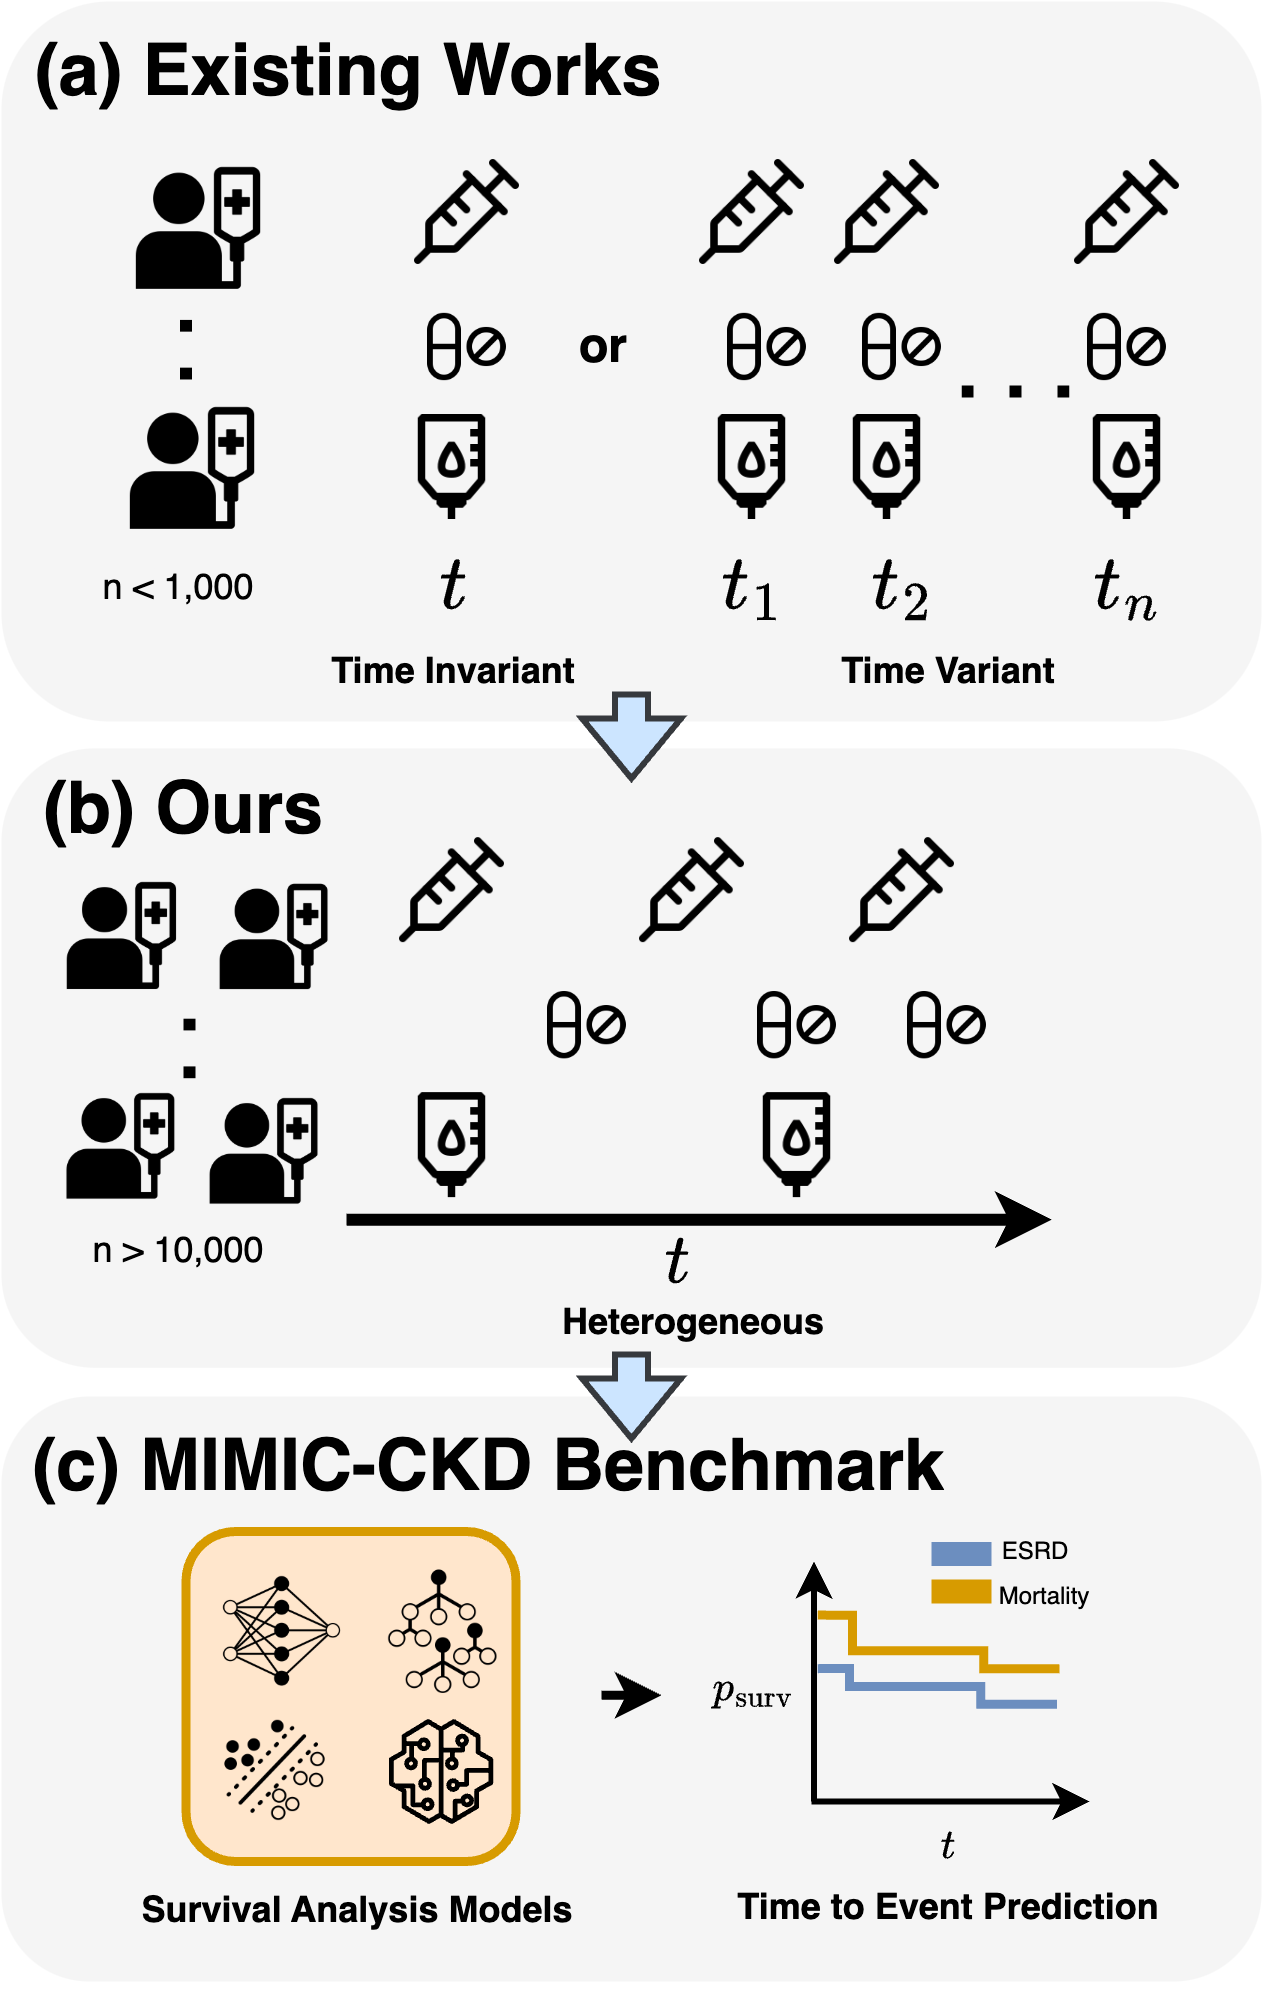
\includegraphics[width=0.45\textwidth]{figs/PatientProfile.drawio.png}
    \caption{Patient profiles are often heterogeneous and complex in clinical settings. They vary considerably in the number of available features and time points of data collection. Leveraging this information to predict CKD progression is nontrivial. (a) In existing works surrounding CKD-ESRD time to event prediction, we observe that many ignore this environment and either assume time invariance \citep{swain2023robust_classifier_imputation_CKD} or uniform monitoring of lab events \citep{chen2019ckd_diagnosis} across a small set of publicly available patient data. (b) Our benchmark explores the challenge of incorporating features that are not only missing across different patient profiles, but also across different time points among a much larger set of patients. (c) We explore the performance of various existing cited survival analysis models in our MIMIC-CKD benchmark.}
    \label{fig:CKD_benchmark}
    \vspace{-0.2cm}
\end{figure}
Chronic kidney disease (CKD) affects over 1 in 7 Americans \citep{CDC2023CKD} and is frequently associated with cardiovascular complications including stroke and heart disease \citep{said2014link_cardiovasc}. CKD can progress to end-stage renal disease (ESRD), which has a five-year survival rate below 50\%. While early intervention is critical for preventing ESRD \citep{levin2011early_detection}, predicting CKD progression remains challenging due to its ambiguous definition and often asymptomatic nature \citep{zhong2017perspective_CKD_biomarkers}.
To identify reliable biomarkers of disease progression, various predictive models have been trained for CKD. In mining electronic health records (EHR) to better understand associated features with CKD, \cite{chicco2021machine_CKD_analysis} find highly correlated biomarkers like age, eGFR, and creatinine, but more remarkably find that other temporally-relevant conditions like hypertension. smoking, and diabetes progression directly affect CKD. The significance of temporal features aligns with evidence that CKD risk increases with age \citep{hill2016global_Survey_CKD}. This temporal dimension is particularly relevant in clinical settings, where kidney function is monitored through recurring blood and urine tests, especially for diabetes-related complications \citep{chen2019ckd_diagnosis}. However, the varying importance of different features across studies highlights a critical gap between controlled research environments and real-world clinical scenarios, where patient data is often heterogeneous and incomplete across time points \citep{wu2024multimodal_missing_modalities} as depicted in Figure \ref{fig:CKD_benchmark}. 

 While many studies have performed CKD survival analysis, their datasets are either private \citep{fatin2023renal_saudi_analysis_example1_of_private_data}, have been conducted on a very small time-invariant scale (i.e less than 1,000 patients) \citep{swain2023robust_classifier_imputation_CKD}, or fail to consider a wider range of features available within EHR.

As such, it is crucial to build a benchmark that leverages a more comprehensive set of features and outcomes. We construct a new dataset analyzing CKD progression from MIMIC-IV \citep{johnson2023mimic_ehr}. 

To the best of our knowledge, our benchmark is the first to:

\begin{itemize}
    \item Include a large-scale cohort of over 10,000 patients across 50,000 clinical visits
    \item Capture realistic patient trajectories through temporally heterogeneous clinical features
\end{itemize}

We benchmark our dataset MIMIC-CKD across a wide variety of methods, including deep neural network survival models that can encode nonlinear relationships between the covariates and predicted outcomes such as DeepHit \citep{lee2018deephit}, Dynamic DeepHit \citep{lee2019dynamic_deephit}, RNN-Surv \citep{giunchiglia2018rnn_surv}, Hazard Transformer \citep{hazard_transformer}, as well as more traditional techniques such as Cox models \citep{cox1972regression}, gradient boosted machines \citep{chen2013gradient_GBSA}, and survival random forests \citep{pickett2021random_survival_forests}. We observe that deep models on average outperform their traditional counterparts and scalably incorporate more features, improving performance upwards of 20\%. 

% \begin{figure*}[h!]
%     \centering
%     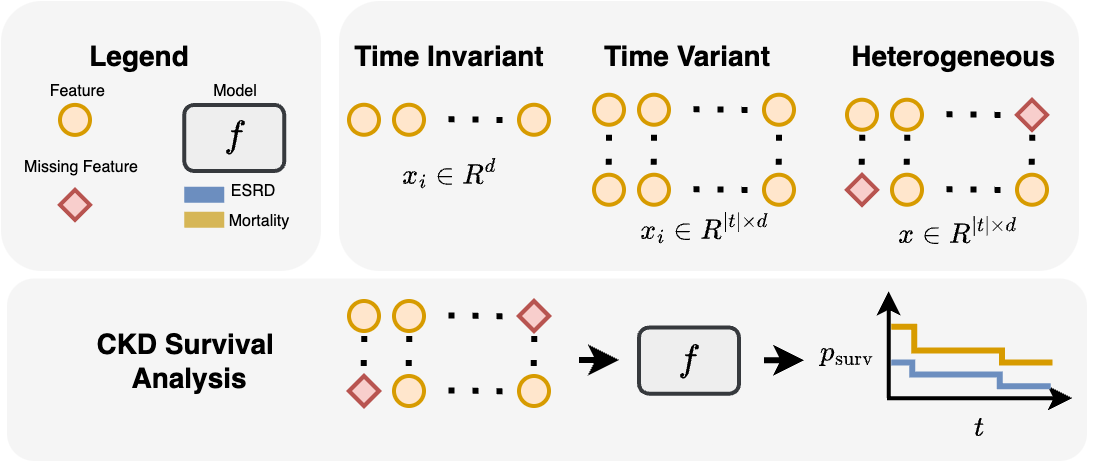
\includegraphics[width=1.0\textwidth]{figs/CKD_Benchmark_Horizontal.drawio.png}
%     \caption{Three scenarios commonly persist in survival analysis works. (1) Time Invariant: There exists no temporal component to co-variates where we effectively take a slice of time for each patient. (2) Time Varying: We take multiple time points and assume all features are visible. (3) Heterogeneous: where we observe both multiple time points and missing features depending on the time point or visit. We note that the large-scale clinical dataset MIMIC and real-world clinical pipelines typically mirror that of the heterogeneous setup \cite{wu2024multimodal_missing_modalities}.}
%     \label{fig:CKD_benchmark}
% \end{figure*}

% insert literature review

% Article on CKD Classificaiton, more related work
% https://pmc.ncbi.nlm.nih.gov/articles/PMC10201999/


% insert literature review of all models that are used here. 
% insert how our model is using those features and more, including the temporal components, and accounting for heterogeneity, which is common in hospital/clinical setings.
\section{Methodology}

\subsection{Problem Formulation} \label{sec: problem formulation}

Time-to-event analysis or survival analysis studies the probability of an event occurring by a given time. We note that this formulation is not unique to the medical field \citep{friedman2015fundamentals_medical_clinical_trials}, and has been applied in business \citep{morrison2004introduction_business} and reliability engineering \citep{pena2004models_reliability_engineering}. Nonetheless, within the medical space and typical EHR systems \citep{kline2022multimodal_medical}, there exist three main data scenarios as depicted in Figure \ref{fig:CKD_benchmark}, each with an additional layer of complexity: time-invariant, time-varying, and heterogeneous.

\textbf{Time invariant and variant eGFR features.} For the time invariant and time variant settings, we use the widely-established estimated glomerular filtration rate (eGFR) as our input biomarker, calculated using the CKD-EPI 2021 equation \citep{omuse2024new_creatinine_epi_equation}:
\begin{align}
\mathrm{eGFR} &= 142 \times \min\left(\frac{\mathrm{Scr}}{\kappa}, 1\right)^{\alpha} \times \max\left(\frac{\mathrm{Scr}}{\kappa}, 1\right)^{-1.2} \nonumber \\
&\quad \times 0.9938^{\mathrm{Age}} \times (1.012)^{\mathrm{I}[\mathrm{Female}]}
\end{align}
where $\mathrm{Scr}$ is serum creatinine (mg/dL), and $\kappa$ and $\alpha$ are gender-specific parameters. 

\textbf{Raw Features.} We also explore time varying the raw features of the equation above as direct inputs rather than weighing it by its previously estimated formulation and compare the predictive performance in Table \ref{tab:stacked_performance_comparison}.

We further describe the three settings in Figure \ref{fig:CKD_benchmark} explored by our benchmark in the subsections below.

\subsubsection{Time Invariant}
In the time-invariant setting, we assume each patient has a snapshot of their profile, regardless of time. In this case, our survival data
\begin{align}
\mathcal{D} = \{(\boldsymbol{x}_i, t_i, e_i)\}_{i=1}^n
\end{align}
is composed of three components where $\boldsymbol{x}_i \in \mathbb{R}^d$ with $d$ the number of features, $t_i \in \mathbb{R}^+$, and $e_i \in \{0,1,\dots,|E|\}$ where $E$ is the set of all competing events (i.e., ESRD, mortality, etc.). When $e_i = 0$, the patient is considered to be right-censored.

In this scenario, the goal is to estimate the hazard function $h(t)$ with our model $f(t)$:
\begin{align}
h(t) = \lim_{\Delta t \to 0} \frac{P(t \leq T < t + \Delta t | T \geq t)}{\Delta t}
\end{align}

Here, $h(t)$ represents the instantaneous rate of event occurrence at time $t$, given that the event has not occurred before time $t$. More specifically, it is the probability that a patient experiences ESRD or death, given they survive up to that time point $t$. In some sense, we are essentially estimating the probability mass function (PMF) of the time-to-event:
\begin{align}
f(t | \boldsymbol{x}) = P(T = t | \boldsymbol{x})
\end{align}

\subsubsection{Time Varying}
However, as suggested in Section 1, most patients were hospitalized multiple times over the course of observation for this dataset. Thus, their profiles consist of multiple snapshots, which is commonly known as time-varying survival analysis \citep{zhang2018time_variant_surv_analysis}. Again, we define our dataset of triples of data, time of event, and event types:
\begin{align}
\mathcal{D} = \{(\boldsymbol{x}_i, t_i, e_i)\}_{i=1}^n
\end{align}
where $\boldsymbol{x}_i \in \mathbb{R}^{s_i \times d}$, $s_i$ is the number of time points observed for individual $i$, $d$ is the feature dimension, and $t_i \in \mathbb{R}^+$. Note that the only difference here is that we have added a sequential component in the data $\boldsymbol{x}_i$.

\subsubsection{Heterogeneous} \label{sec: Heterogeneous}
In the heterogeneous setting, we build upon the time-varying framework but account for missing features across different time points. Our dataset structure remains similar:
$\mathcal{D} = \{(\boldsymbol{x}_i, t_i, e_i)\}_{i=1}^n$
where $\boldsymbol{x}_i \in \mathbb{R}^{s_i \times d}$, with $s_i$ representing the number of observed time points for individual $i$, and $d$ is the feature dimension. However, unlike the time-varying setting, not all features are observed at each time point, resulting in a sparse representation. Formally, we can represent this as a mask $\boldsymbol{m}_i \in \{0,1\}^{s_i \times d}$ where $m_{i,j,k} = 0$ indicates that feature $k \in \{1, \dots, d\}$ at time point $j \in \{1, \dots, s_i\}$ for individual $i$ is missing.

In our specific implementation, each input representation for patient $i$ at time $j$ includes 2 types of features, eGFR and Hemoglobin with 4 columns to represent missing features: $\mathbf{x}_{i,j} = (\text{eGFR}_{i,j}, I^{(m)}_{\text{eGFR},i,j}, P_{i,j}, I^{(m)}_{P,i,j}, A_{i,j}, I^{(m)}_{A,i,j})$ where $I^{(m)}_{\text{eGFR},i,j} \in \{0,1\}$ indicates that $\text{eGFR}_{i,j}$ is missing when equal to 1 (similarly for $I^{(m)}_{P,i,j}$ and $I^{(m)}_{A,i,j}$). Here, $P_{i,j}$ represents proteinuria measurement for patient $i$ at time $j$, $A_{i,j}$ represents serum albumin level for patient $i$ at time $j$, and $I^{(m)}_{\cdot,i,j}$ denotes the missing data indicator with superscript $(m)$ for "missing".



% This setting better reflects real-world clinical scenarios, particularly in datasets like MIMIC, where patients undergo different tests and procedures at varying time points based on their condition and clinical necessity. The challenge in this framework extends beyond modeling temporal dynamics to also handling the missing information across the feature space.

Models designed for this setting must account for both the temporal evolution of patient states and the informativeness of the missing pattern itself, as the absence of certain measurements may carry clinical significance (e.g., tests not ordered because the clinician deemed them unnecessary based on other observations). Nonetheless, in our benchmark, we note that this representation is not fixed, and should be explored in future work.

\subsection{Benchmarked Models} \label{sec:models}

In this subsection, we introduce each model evaluated in our survival analysis experiments across the different data scenarios described above.

\subsubsection{Traditional Survival Analysis Models}
We include two parametric/nonparametric baseline models, implemented via the lifelines Python package \citep{davidson2019lifelines}.

\textbf{Cox Proportional Hazards Model} \citep{cox1972regression} models the hazard function as:
\begin{align}
\lambda(t \mid \mathbf{x}) = \lambda_0(t)\,\exp\bigl(\mathbf{x}^\intercal \boldsymbol{\beta}\bigr)
\end{align}
where $\lambda_0(t)$ is the baseline hazard function and $\boldsymbol{\beta}$ represents the coefficients that quantify the effect of covariates $\mathbf{x}$ on the hazard. The model is trained by maximizing the partial likelihood:
\begin{align}
L(\boldsymbol{\beta}) = \prod_{i:e_i=1} \frac{\exp(\boldsymbol{\beta}^\intercal \mathbf{x}_i)}{\sum_{j:t_j \geq t_i} \exp(\boldsymbol{\beta}^\intercal \mathbf{x}_j)}
\end{align}

We use the lifeline implementation for time invariant and time variant scenarios.
% Then use it like this:
% \begin{lstlisting}[language=Python]
% from lifelines import CoxPHFitter
% from lifelines import CoxTimeVaryingFitter
% \end{lstlisting}

\textbf{Weibull Accelerated Failure Time (AFT)} model \citep{anderson1991nonproportional_weibull} parameterizes the survival function as:
\begin{align}
S(t \mid \mathbf{x}) = \exp\left(-\left(\frac{t}{\lambda(\mathbf{x})}\right)^{\rho}\right)
\end{align}
where $\lambda(\mathbf{x}) = \exp(\mathbf{x}^\intercal \boldsymbol{\beta})$ is the scale parameter and $\rho$ is the shape parameter. Implemented as \texttt{from lifelines import WeibullAFTFitter}, we estimate regression coefficients $\boldsymbol{\beta}$ and shape parameter $\rho$. Continuous covariates are standardized; categorical covariates are one-hot encoded.

% The fundamental difference between the Cox and Weibull models lies in their modeling approach: while the Cox model directly models the hazard rate $\lambda(t \mid \mathbf{x})$ without specifying the baseline hazard distribution, the Weibull AFT model assumes a specific parametric form for the entire survival distribution. This parametric assumption allows the Weibull model to directly predict survival times, whereas the Cox model primarily estimates relative risks and requires additional steps to obtain absolute survival probabilities or time predictions.

\subsubsection{Deep Survival Analysis Models}

Recent years have seen a surge in deep learning approaches for survival analysis, capable of handling complex data structures and relationships. All deep architectures consume time-indexed feature tensors $x_i \in \mathbb{R}^{s_i\times d}$ as described in the experimental settings.

\textbf{DeepSurv} \citep{katzman2018deepsurv} is a feedforward implementation of the Cox model with fully connected layers. We modify the original implementation to handle time-varying inputs by stacking each visit as a separate "instance" and encoding time-to-event as an additional feature. The network has three hidden layers (ReLU activations, size 128) followed by a linear output layer representing the log-hazard. We use Cox partial log-likelihood as the loss.

\textbf{DeepHit} \citep{lee2018deephit} directly estimates the joint distribution of survival times and competing events without assuming any specific form for the underlying stochastic process. It employs a neural network architecture with a shared subnetwork and cause-specific subnetworks to model the discrete probability mass function:
\begin{align}
P(T=t, E=k|\boldsymbol{x}) = y_{t,k}
\end{align}
where $y_{t,k}$ is the output of the network for time $t$ and event $k$. The model is trained using a composite loss function:
\begin{align}
L_{total} = L_1 + \alpha L_2
\end{align}
where $L_1$ is the negative log-likelihood term accounting for right censoring:
\begin{align}
L_1 &= -\sum_{i=1}^n \left[ \mathbf{1}_{(e_i \neq 0)} \log(y_{t_i,e_i}) \right. \nonumber \\
&\quad + \left. \mathbf{1}_{(e_i = 0)} \log\left(1 - \sum_{k=1}^K \sum_{t \leq t_i} y_{t,k}\right) \right]
\end{align}
and $L_2$ is a ranking loss that encourages proper ordering of events:
\begin{align}
L_2 = \sum_{k=1}^K \sum_{i,j: e_i=k, t_i<t_j} \sigma\left(\hat{F}_k(t_i|\boldsymbol{x}_j) - \hat{F}_k(t_i|\boldsymbol{x}_i)\right)
\end{align}
Here, $\hat{F}_k(t|\boldsymbol{x})$ is the estimated cumulative incidence function for event $k$ up to time $t$ given covariates $\boldsymbol{x}$, and $\sigma$ is a smoothing function. This composite loss formulation has inspired many subsequent deep survival models.

\textbf{Dynamic-DeepHit} \citep{lee2020dynamicdeephit} extends DeepHit to irregularly sampled time series. At each timestep we feed $\{\mathbf{x}_{i,j}, m_{i,j}, \Delta t_{i,j}\}$ where $\Delta t_{i,j} = t_{i,j} - t_{i,j-1}$. The architecture comprises a shared MLP encoder, a bi-directional LSTM layer, and cause-specific MLP heads that output discrete hazard probabilities over pre-specified time bins. The model uses the combined log-likelihood and ranking loss from DeepHit, tuning coefficient $\alpha \in [0.1, 1.0]$.

\textbf{RNN-Surv} \citep{martinez2020rnnsurv} uses gated recurrent units (GRUs) to model temporal dependencies and outputs risk scores for each patient at each visit. The architecture includes an input embedding layer projecting $\mathbb{R}^d \to \mathbb{R}^{64}$, two-layer GRU (hidden size 64), and a time-to-event decoder mapping the last hidden state to a scalar risk score. Different from Dynamic-DeepHit, RNN-Surv model employs the traditional negative Cox partial log-likelihood on final risk scores. 
% \citep{nagpal2021hazard}

\textbf{LogisticHazard} implements a discrete‐time survival model by framing event hazards in logistic form. Time is first divided into a fixed number of intervals, and for each interval the model learns the log-odds of "failure" versus "survival" in that window. Under the hood it's a neural network whose final layer outputs one logit per time interval; training minimizes the negative log‐likelihood of the observed interval‐censored outcomes. This approach marries classic discrete‐time hazard modeling with the flexibility of deep nets, allowing rich feature representations, non‐linear covariate effects, and end-to-end learning of survival curves directly from data.

\textbf{Hazard Transformer.} Inspired by the original Transformer model\citep{vaswani2017attention}, the Hazard Transformer \citep{hazard_transformer} replaces RNNs with the self-attention mechanism. It consists of positional encoding added to each $\mathbf{x}_{i,j}$, two Transformer encoder blocks (4 heads, hidden size 64; feedforward sublayers size 128), and a final linear layer producing discrete hazard probabilities over pre-binned intervals. The model uses cross-entropy-based ranking loss inspired by the DeepHit framework, with dropout 0.2 on attention and feedforward layers.

\subsubsection{Ensemble-Learning-Based Models}

We evaluated two tree-based survival learners from `scikit-survival`:

\textbf{Gradient Boosting Survival Analysis (GBSA)} \citep{chen2013gradient_GBSA} offers a powerful nonparametric alternative that can capture complex, non-linear relationships without imposing restrictive assumptions on the hazard function form. The objective function approximates the Cox model through additive ensemble learning:
\begin{align}
L = \sum_i \ell(y_i, \hat{y}_i) + \Omega(f)
\end{align}
where $\ell$ is the negative log partial likelihood and $\Omega(f)$ is regularization. For brevity's sake, we defer to the literature for their exact details.

\textbf{Random Survival Forest (SRF)} \citep{pickett2021random_survival_forests, ishwaran2008random} extends random forests to survival data. Implemented as \texttt{sksurv.ensemble.RandomSurvivalForest}, it uses Harrell's concordance index (C-index) on out-of-bag samples to guide hyperparameter selection. Again, we defer to the literature for their exact implementation. 

\textbf{FastSurvivalSVM} adapts support vector machines to right‐censored survival data by optimizing a convex surrogate for the concordance index. It learns a linear ranking function over feature space that pushes subjects with earlier events to have higher "risk scores" than those with later or censored times, subject to margin constraints and regularization.

\subsection{Model Training and Optimization}

\textbf{Hyperparameter Tuning for Deep Models:} For RNN-based and Transformer architectures, we perform Bayesian hyperparameter optimization using Optuna with 10 trials and 50 epochs per trial. Learning rates are tuned in log-uniform range $[10^{-5}, 10^{-2}]$, dropout rates in $[0.1, 0.5]$, and weight decay in $[10^{-6}, 10^{-3}]$.

\textbf{Ensemble Model Tuning:} For GBSA and SRF, we perform grid search over number of trees, learning rates, max depths, and minimum samples split parameters.

\textbf{Data Preprocessing:} Categorical variables are one-hot encoded, and we use an 80/20 train/test split by patient ID to ensure generalization capability. Traditional models use default optimization routines, deep models use Adam with early stopping, and ensemble models use validation-based selection.
\section{Results}
% \begin{table}[htbp]
% \centering
% \begin{tabular}{llll}
%  & & \multicolumn{2}{c}{\textbf{All CKD stage 3-5 (n=10179)}}\\
% \hline
% \textbf{Characteristics} & \textbf{All CKD (n=22336)} & \textbf{Non-ESRD (n=2790)}& \textbf{ESRD (n=7389)}\\
% \hline
% \multicolumn{4}{l}{\textbf{Demographics}} \\
% Age (years) & 71.1 $\pm$ 14.3 & 74.795 $\pm$ 12.470& 71.774 $\pm$ 13.668\\
% Gender & M: 13223, F: 9113 & M: 1555, F:1235& M: 4247, F: 3142\\
% \hline
% \multicolumn{4}{l}{\textbf{Clinical Characteristics}} \\
% CKD Stage 3-5, n (\%) & 10179 (45.6) & -& -\\
% Hypertension, n (\%) & 10531 (47.1) & 1418  (50.824)& 4317 (58.425)\\
% Diabetes Mellitus, n (\%) & 4954 (22.2) & 565 (20.251)& 2288 (30.965)\\
% \hline
% \multicolumn{4}{l}{\textbf{Laboratory Parameters}} \\
% Serum Creatinine (mg/dL) & 2.256 $\pm$ 1.756 & 2.126 $\pm$ 2.026& 2.27 $\pm$ 1.723\\
% eGFR (mL/min/1.73m²) & 41.502 $\pm$ 23.532 & 46.4 $\pm$ 24.35& 40.968 $\pm$ 23.379\\
% Proteinuria (g/24 hours) & 0.836 (2.474)* & 0.837 (2.294)*& 0.458 (4.319)*\\
% \hline
% \multicolumn{4}{l}{\textbf{Medication Use}} \\
% ACE Inhibitors or ARBs, n (\%) & 8633 (38.7) & 954 (34.194)& 3221 (43.592)\\
% \hline
% \multicolumn{4}{l}{\small *Values presented as median (IQR)} \\
% \end{tabular}
% \caption{Baseline Characteristics by ESRD Status. Patients are stratified by whether they developed ESRD during follow-up. We investigate a wide variety of useful features defined by \citep{zhong2017perspective_CKD_biomarkers} and more recently \citep{dana2024integratedmachinelearningsurvival_feature_analysis}. We investigate these features across time. We also investigate features that may not necessarily be omnipresent across all time points.}
% \label{tab:baseline_characteristics}
% \end{table}

\begin{table}[h]
\centering
\resizebox{0.5\textwidth}{!}{%
\begin{tabular}{lcc}
\hline
\textbf{} & \textbf{Non-ESRD} & \textbf{ESRD} \\
\hline
\multicolumn{3}{l}{\textbf{Patient Demographics}} \\
\quad \# of Patients & 2,790 & 7,389 \\
\quad Age (years) & 74.8 ± 12.5 & 71.8 ± 13.7 \\
\quad Male & 55.7\% & 57.5\% \\
\quad Hypertension & 50.8\% & 58.4\% \\
\quad Diabetes mellitus & 20.3\% & 31.0\% \\
\quad ACE inhibitor/ARB use & 34.2\% & 43.6\% \\
\quad \# of admissions & 6,773& 47,441\\
\hline
\multicolumn{3}{l}{\textbf{Laboratory Values}} \\
\quad Serum creatinine (mg/dL) & 2.1 ± 2.0 & 2.3 ± 1.7 \\
\quad eGFR (mL/min/1.73m²) & 46.4 ± 24.4 & 41.0 ± 23.4 \\
\quad Proteinuria (g/24h)* & 0.8 [2.3] & 0.5 [4.3] \\
\hline
\end{tabular}%
}
\caption{Baseline Characteristics of CKD Stage 3-5 Patients by ESRD Status. This analysis focuses exclusively on patients with chronic kidney disease stages 3-5 (n=10,179), stratified by whether they developed end-stage renal disease (ESRD) during follow-up. Continuous variables are presented as mean ± standard deviation, except for proteinuria which is presented as median with interquartile range due to its skewed distribution. We investigate a wide variety of useful features defined by \citep{zhong2017perspective_CKD_biomarkers} and more recently \citep{dana2024integratedmachinelearningsurvival_feature_analysis}. We investigate these features across time. We also investigate features that may not necessarily be omnipresent across all time points.}
\label{tab:baseline_characteristics}
\end{table}

\subsection{Dataset Statistics}
Given that ESRD risks are substantially higher in later CKD stages \citep{sud2014ckd_esrd_at_stage3_5}, we identified 10,179 patients with stage 3--5 CKD, of whom 7,389 progressed to ESRD. As shown in Table~\ref{tab:baseline_characteristics}, ESRD patients were younger, had higher rates of diabetes and hypertension, more severe renal dysfunction, and increased use of renin--angiotensin inhibitors compared to non-progressors, establishing clinically meaningful baseline differences for model comparison.

\textbf{Evaluation metrics.} We benchmark our survival analysis models using three conventional metrics: concordance index (C-index) \citep{longato2020practical_c_index}, Brier score \citep{assel2017brier}, and area under the ROC curve (AUC) \citep{huang2005using_AUC}.

\subsection{Time Invariant}
We benchmark several traditional time-invariant models for CKD survival analysis as discussed in Section \ref{sec:models}. Specifically, we evaluate traditional models (Cox proportional hazards, Weibull), ensemble methods (gradient boosted survival analysis or GBSA, survival random forests or SRF), and the neural network-based DeepSurv model.

% Time-Invariant Models Table
% \begin{table}[h!]
%     \centering
%     \begin{tabular}{lccc}
%         \toprule
%         \textbf{Model} & \textbf{C-Index} & \textbf{Brier score} & \textbf{AUC} \\
%         \midrule
%         Cox & 0.517±0.008  &   0.443±0.001   &  0.527±0.012 \\
%         DeepSurv & \textbf{0.523±0.002}   &  0.475±0.012  &   0.464±0.002 \\
%         GBSA & 0.523±0.011  &   0.329±0.043   &  0.534±0.016 \\
%         SRF & 0.517±0.006  &   0.502±0.004  &   0.527±0.009 \\
%         Weibull & 0.521±0.001   &  0.485±0.007   &  \textbf{0.535±0.001} \\
%         LogisticHazard & 0.514±0.010  &   \textbf{0.566±0.008}  &   0.496±0.023 \\
%         Fast Survival SVM & 0.510±0.007  &   0.252±0.004  &   0.485±0.010 \\
%         \bottomrule
%     \end{tabular}
%     \caption{Performance of Time-Invariant Models. Models use static patient snapshots without longitudinal information. Bold values indicate best performance for each metric.}
%     \label{tab:time_invariant_performance}
% \end{table}
\begin{table}[h!]
    \centering
    \footnotesize % Smaller font size
    \resizebox{0.5\textwidth}{!}{% Resize to fit textwidth
    \begin{tabular}{@{}lccc@{}}
        \toprule
        \textbf{Model} & \textbf{C-Index} $\uparrow$ & \textbf{Brier score} $\downarrow$ & \textbf{AUC} $\uparrow$ \\
        \midrule
        Cox & 0.517±0.008 & 0.443±0.001 & 0.527±0.012 \\
        DeepSurv & \textbf{0.523±0.002} & 0.475±0.012 & 0.464±0.002 \\
        GBSA & 0.523±0.011 & 0.329±0.043 & 0.534±0.016 \\
        SRF & 0.517±0.006 & 0.502±0.004 & 0.527±0.009 \\
        Weibull & 0.521±0.001 & 0.485±0.007 & \textbf{0.535±0.001} \\
        LogisticHazard & 0.514±0.010 & 0.566±0.008 & 0.496±0.023 \\
        Fast Survival SVM & 0.510±0.007 & \textbf{0.252±0.004} & 0.485±0.010 \\
        \bottomrule
    \end{tabular}
    } % End resizebox
    \caption{Performance of Time-Invariant Models. Models use static patient snapshots without longitudinal information. Bold values indicate best performance for each metric.}
    \label{tab:time_invariant_performance}
\end{table}

\textbf{More complex and less interpretable models do not provide any significant benefits in time invariant settings.} At the cost of explainability, we see a small improvement in DeepSurv over the Cox model in C-index. However, the interpretable Weibull model is comparable and better depending on the metric. Nonetheless, traditional models like the Cox or Weibull model seem comparable in performance to the less interpretable SRF, GBSA, and DeepSurv models when considering both metrics.


\subsection{Time Variant and Heterogeneous Scenarios}
To understand the predictive capababilites of survival analysis models under different time variant settings, we benchmarked 4 models. Namely, we benchmark the Cox model, and a variety of deep architectures such as Dynamic-DeepHit \citep{lee2019dynamic_deephit}, Hazard Transformer \citep{hazard_transformer}, and RNN-Surv \citep{martinez2020rnnsurv}. 

\begin{table}[h!]
    \centering
    \footnotesize
    \resizebox{0.5\textwidth}{!}{%
    \begin{tabular}{@{}l*{3}{c}@{}}
        \toprule
        \multicolumn{4}{c}{\textbf{Time-Variant (Baseline)}} \\
        \midrule
        \textbf{Model} & \textbf{C-Index} $\uparrow$ & \textbf{Brier} $\downarrow$ & \textbf{AUC} $\uparrow$ \\
        \midrule
        Cox & 0.545±0.001 & 0.215±0.002 & 0.539±0.002 \\
        Dynamic-DeepHit & \textbf{0.735±0.069} & \textbf{0.036±0.003} & \textbf{0.798±0.197} \\
        Hazard Transformer & 0.500±0.000 & 0.566±0.007 & 0.500±0.000 \\
        RNNSurv & 0.640±0.076 & 0.082±0.088 & 0.648±0.080 \\
        Logistic Hazard & 0.514±0.010 & 0.566±0.008 & 0.496±0.023 \\
        \midrule
        \multicolumn{4}{c}{\textbf{Time-Variant Raw}} \\
        \midrule
        \textbf{Model} & \textbf{C-Index} $\uparrow$ & \textbf{Brier} $\downarrow$ & \textbf{AUC} $\uparrow$ \\
        \midrule
        Cox & \textcolor{red}{0.374±0.004} $\downarrow$ & \textcolor{red}{0.926±0.029} $\uparrow$ & \textcolor{red}{0.352±0.004} $\downarrow$ \\
        Dynamic-DeepHit & \textcolor{green}{0.780±0.065} $\uparrow$ & \textcolor{gray}{0.037±0.002} $=$ & \textcolor{green}{0.830±0.187} $\uparrow$ \\
        Hazard Transformer & \textcolor{gray}{0.500±0.000} $=$ & \textcolor{gray}{0.566±0.007} $=$ & \textcolor{gray}{0.500±0.000} $=$ \\
        RNNSurv & \textcolor{green}{0.668±0.042} $\uparrow$ & \textcolor{gray}{0.096±0.057} $=$ & \textcolor{green}{0.681±0.040} $\uparrow$ \\
        Logistic Hazard & \textcolor{gray}{0.507±0.016} $=$ & \textcolor{gray}{0.566±0.007} $=$ & \textcolor{gray}{0.513±0.021} $=$ \\
        \midrule
        \multicolumn{4}{c}{\textbf{Heterogeneous Features}} \\
        \midrule
        \textbf{Model} & \textbf{C-Index} $\uparrow$ & \textbf{Brier} $\downarrow$ & \textbf{AUC} $\uparrow$ \\
        \midrule
        Cox & \textcolor{red}{0.406±0.003} $\downarrow$ & \textcolor{red}{0.294±0.007} $\uparrow$ & \textcolor{red}{0.389±0.003} $\downarrow$ \\
        Dynamic-DeepHit & \textcolor{green}{0.761±0.014} $\uparrow$ & \textcolor{red}{0.056±0.000} $\uparrow$ & \textcolor{red}{0.492±0.047} $\downarrow$ \\
        Hazard Transformer & \textcolor{gray}{0.500±0.000} $=$ & \textcolor{red}{0.546±0.000} $\downarrow$ & \textcolor{gray}{0.500±0.000} $=$ \\
        RNNSurv & \textcolor{green}{0.647±0.002} $\uparrow$ & \textcolor{red}{0.127±0.043} $\uparrow$ & \textcolor{green}{0.651±0.003} $\uparrow$ \\
        Logistic Hazard & \textcolor{gray}{0.518±0.008} $=$ & \textcolor{red}{0.529±0.027} $\uparrow$ & \textcolor{gray}{0.526±0.015} $=$ \\
        \bottomrule
    \end{tabular}
    }
    \caption{Stacked Performance Comparison Across Settings. Time-Variant serves as baseline. Green indicates improvement ($>0.02$ difference), red indicates degradation ($>0.02$ difference), gray indicates no significant change ($\leq 0.02$ difference). For C-Index and AUC, higher is better ($\uparrow$); for Brier score, lower is better ($\downarrow$). Dynamic-DeepHit shows consistent strong performance across all settings and sees upwards of a 4\% performance improvement in the raw setting.}
    \label{tab:stacked_performance_comparison}
\end{table}

% \begin{table*}[h!]
%     \centering
%     \footnotesize
%     \resizebox{\textwidth}{!}{%
%     \begin{tabular}{@{}l*{6}{c}@{}}
%         \toprule
%         & \multicolumn{3}{c}{\textbf{Time-Variant}} & \multicolumn{3}{c}{\textbf{Time-Variant Raw}} \\
%         \cmidrule(lr){2-4} \cmidrule(lr){5-7}
%         \textbf{Model} & \textbf{C-Index} $\uparrow$ & \textbf{Brier} $\downarrow$ & \textbf{AUC} $\uparrow$ & \textbf{C-Index} $\uparrow$ & \textbf{Brier} $\downarrow$ & \textbf{AUC} $\uparrow$ \\
%         \midrule
%         Cox & 0.545±0.001 & 0.215±0.002 & 0.539±0.002 & 0.374±0.004 & 0.926±0.029 & 0.352±0.004 \\
%         Dynamic-DeepHit & \textbf{0.735±0.069} & \textbf{0.036±0.003} & \textbf{0.798±0.197} & \textbf{0.780±0.065} & \textbf{0.037±0.002} & \textbf{0.830±0.187} \\
%         Hazard Transformer & 0.500±0.000 & 0.566±0.007 & 0.500±0.000 & 0.500±0.000 & 0.566±0.007 & 0.500±0.000 \\
%         RNNSurv & 0.640±0.076 & 0.082±0.088 & 0.648±0.080 & 0.668±0.042 & 0.096±0.057 & 0.681±0.040 \\
%         Logistic Hazard & 0.514±0.010 & 0.566±0.008 & 0.496±0.023 & 0.507±0.016 & 0.566±0.007 & 0.513±0.021 \\
%         \bottomrule
%     \end{tabular}
%     }
%     \caption{Performance of Longitudinal Models: Time-Variant vs Time-Variant Raw. Time-variant include eGFR across multiple time points. Time-variant raw decomposes eGFR into its input components and feeds those into the models. Dynamic-DeepHit performs best across both settings.}
%     \label{tab:time_variant_performance}
% \end{table*}
% \begin{table}[h!]
%     \centering
%     \footnotesize
%     \resizebox{0.5\textwidth}{!}{%
%     \begin{tabular}{@{}l*{3}{c}@{}}
%         \toprule
%         \textbf{Model} & \textbf{C-Index} $\uparrow$ & \textbf{Brier} $\downarrow$ & \textbf{AUC} $\uparrow$ \\
%         \midrule
%         Cox & 0.406±0.003  &   0.294±0.007   &  0.389±0.003 \\
%         Dynamic-DeepHit & \textbf{0.761±0.014}  &   \textbf{0.056±0.000}  &   0.492±0.047 \\
%         Hazard Transformer & 0.500±0.000 & 0.546±0.000 & 0.500±0.000 \\
%         RNNSurv & 0.647±0.002  &   0.127±0.043  &   \textbf{0.651±0.003} \\
%         Logistic Hazard & 0.518±0.008  &   0.529±0.027  &   0.526±0.015 \\
%         \bottomrule
%     \end{tabular}
%     }
%     \caption{Performance of Longitudinal Models: Heterogeneous Setting. This setting incorporates heterogeneous features like Albumin and protein measurements alongside eGFR. RNNSurv performs best for C-Index and AUC, while Cox regression achieves the best Brier score.}
%     \label{tab:heterogeneous_performance}
% \end{table}

\textbf{Incorporating temporal features improves performance, but only when models can effectively leverage them.} We observe that while the Cox model benefits from additional time points in the time-variant setting, the improvement is modest—approximately 3\% increase in predictive performance. In contrast, deep architectures such as Dynamic-DeepHit and RNNSurv achieve substantial performance gains exceeding 20\%. Notably, the transformer architecture underperforms across all metrics, yielding results worse than even time-invariant models. This poor performance of our Hazard Transformer aligns with existing literature, as transformers typically require advanced training techniques or extensive feature engineering to effectively model time-series data \citep{wen2023transformerstimeseriessurvey}.

% \textbf{The effectiveness of eGFR versus its constituent covariates varies by model architecture.} As shown in Table \ref{tab:stacked_performance_comparison}, our best-performing model, Dynamic-DeepHit, derives the greatest benefit from using eGFR as an input feature. The Cox model experiences severe performance degradation when using raw features instead of the computed eGFR directly. However, this pattern reverses with RNN-Surv, where raw features yield superior, albeit not by a significant margin (4.373\% improvement in C-index), results. Nonetheless, Dynamic-DeepHit seems to be a consistently top-performer in our benchmark.
\textbf{eGFR is a flawed composite feature.} While eGFR is commonly used in clinical settings, its formulation is not necessarily optimal. In fact, models can directly learn relationships between eGFR components, as evidenced by improved performance in Dynamic DeepHit and RNNSurv. In contrast, more interpretable and linear models like our Cox baseline show substantial performance declines. This observation makes sense because the eGFR equation essentially functions as a form of feature engineering, with explicitly defined weights for each component.
% Features such as albumin and urine protein measurements are routinely collected for CKD patients \citep{coresh2005proteinuria} \citep{martin2011laboratory_urine_proteinuria_CKD} due to their established clinical significance as key biomarkers for CKD progression and ESRD risk.

\textbf{Current survival analysis models struggle to effectively utilize heterogeneous clinical features.} Features like hemoglobin are commonly collected from CKD patients since anemia is a common CKD complication \cite{atkinson2018anemia}. However, Table \ref{tab:stacked_performance_comparison} reveals that incorporating these heterogeneous features produces negligible improvements or actual performance decreases. This limitation represents an important challenge requiring further investigation in model architecture design and remains an active research area in healthcare AI systems.

While Dynamic DeepHit shows C-index improvements, suggesting better risk ranking across patient cohorts, its substantial drops in AUC and Brier scores indicate that heterogeneous features result in poorly calibrated models. Every model shows declining Brier scores, suggesting that while relative ranking predictions remain unchanged, incorporating heterogeneous inputs severely disrupts model calibration.

\subsection{Feature Analysis}
We run a feature analysis to better understand the importance of each input feature across both our raw and heterogeneous scenarios. In particular, we want to understand what features is driving each model's predictions as shown in Figures \ref{fig:Feature_Analysis_Raw} and \ref{fig:Feature_Analysis_Hetero}. 

\textbf{Static features are still highly relevant for time-series predictive performance.} Remarkably in Figure \ref{fig:Feature_Analysis_Raw}, our best performing model Dynamic DeepHit weighs static characteristics such as gender and age just as important as serum creatinine. 

\textbf{Missing features highly affect performance within our models.} We include a missing feature indicator as part of our feature set in our heterogeneous case across different time points. In Figure \ref{fig:Feature_Analysis_Hetero}, we observe that across all models our "missing" features are highly relevant in downstream predictions. 

\begin{figure}[h!]
    \centering
    \vspace{-0.2cm}
    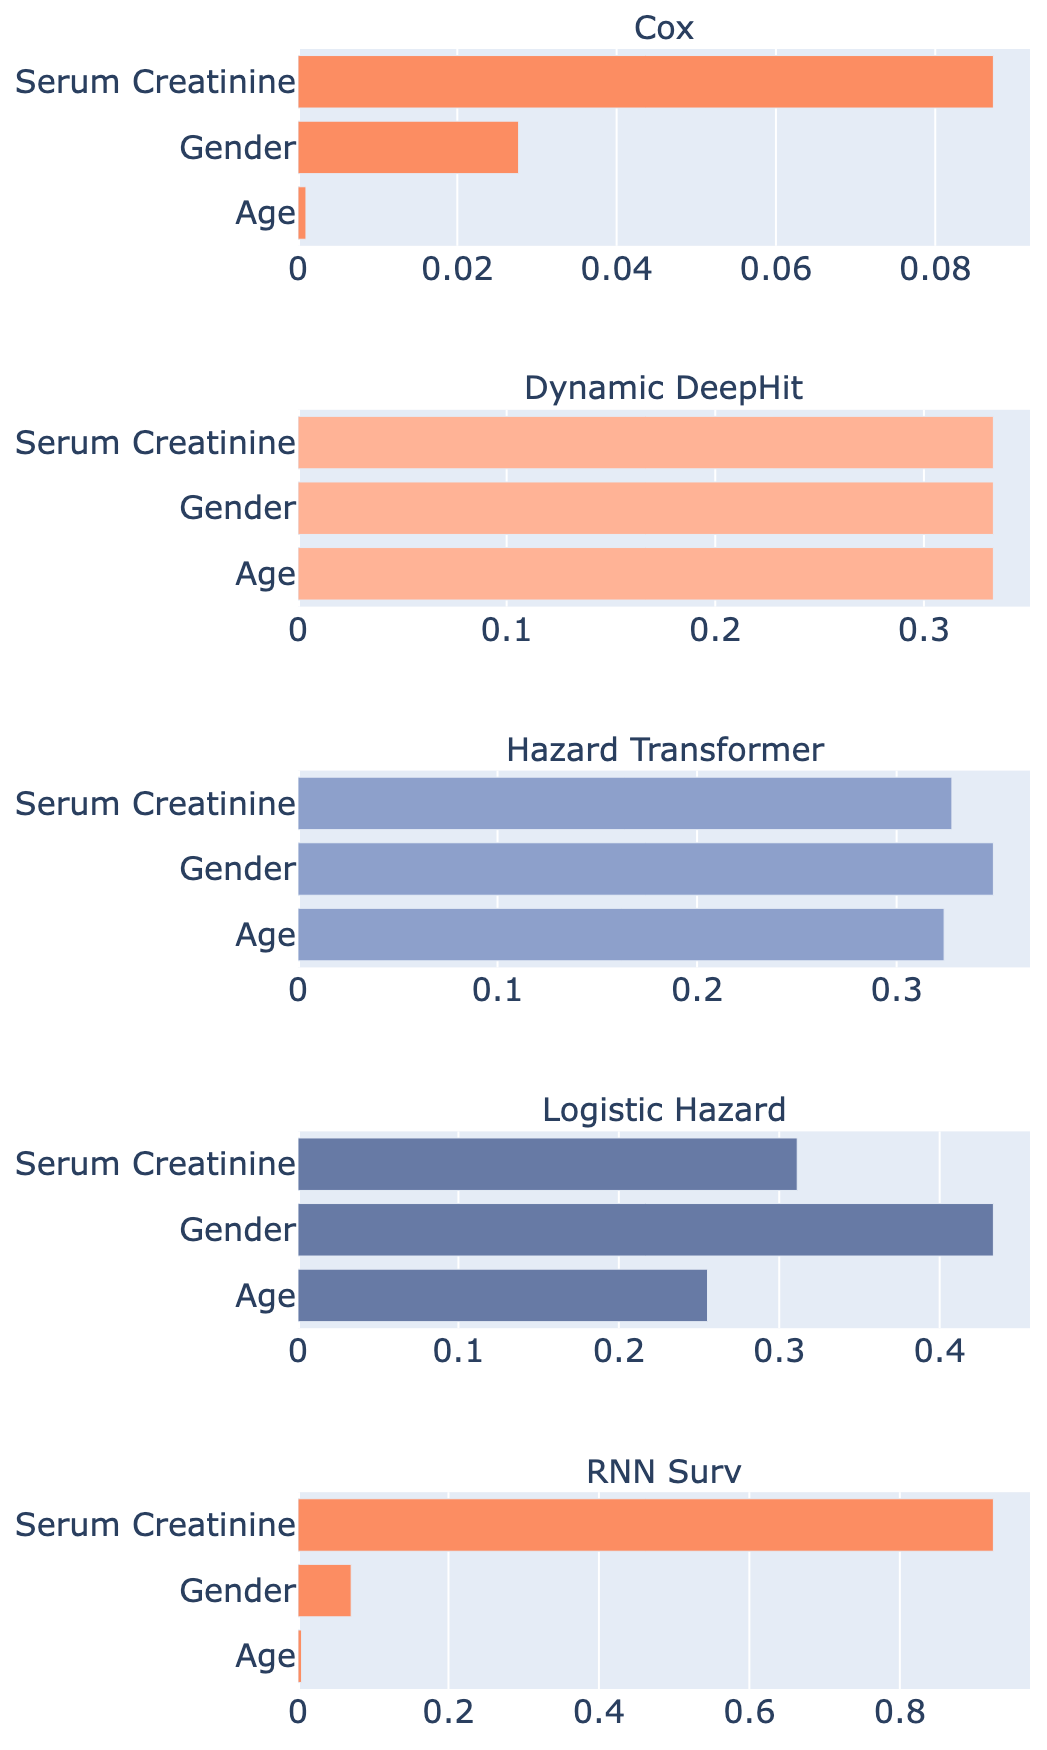
\includegraphics[width=0.5\textwidth]{figs/raw_feature_importance_individual.png}
    \caption{Feature Importance of the "Raw" Setting. We explore how directly inputting the individual components of the eGFR equation drives performance Here, we plot our Cox model's weight coefficients along with the gradient-based saliency maps \citep{simonyan2014deepinsideconvolutionalnetworks_cnn} across our neural baselines. We observe that serum creatinine is highly relevant across all models, but age and gender varies depending on the model.}
    \label{fig:Feature_Analysis_Raw}
    \vspace{-0.2cm}
\end{figure}

\begin{figure}[h!]
    \centering
    \vspace{-0.2cm}
    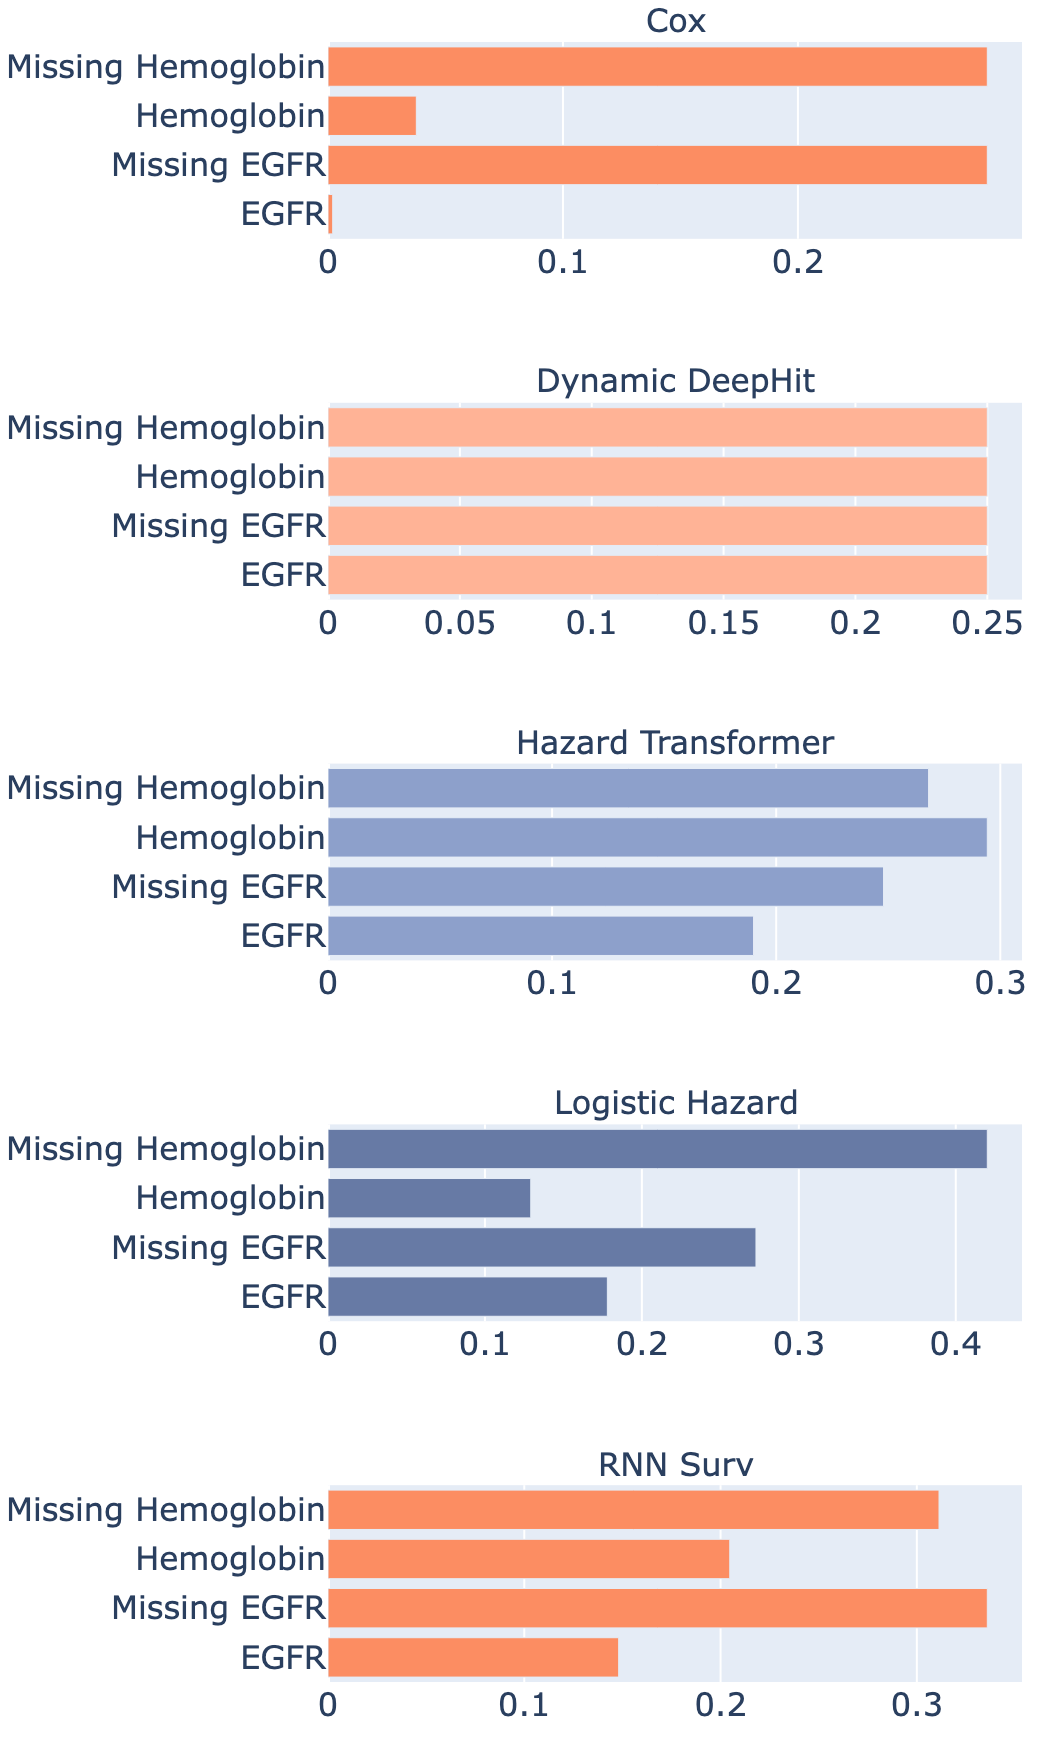
\includegraphics[width=0.5\textwidth]{figs/feature_importance_individual.png}
    \caption{Feature Importance Within The Heterogeneous Setting. We explore how (missing) features affect downstream performance by running a feature analysis. Here, we plot our Cox model's weight coefficients along with the gradient-based saliency maps \citep{simonyan2014deepinsideconvolutionalnetworks_cnn} with respect to each input feature across our neural baselines. We observe that missing features have a massive effect on model predictions.}
    \label{fig:Feature_Analysis_Hetero}
    \vspace{-0.2cm}
\end{figure}




% \subsection{Time Invariant Modeling}
% We first evaluated each model in a time-invariant setting, representing each patient by a single static snapshot. Overall discrimination was modest: no model achieved a C-index above 0.53 or an AUC above 0.54 (Table 2):contentReference[oaicite:1]{index=1}. DeepSurv achieved the highest C-index (0.526), whereas the Weibull model yielded the best AUC (0.537).

% \begin{table}[h]
%     \centering
%     \begin{tabular}{lcc}
%         \toprule
%         Model Name & C-Index & Brier score &AUC\\
%         \midrule
%         Cox & 0.503 & 0.504\\
%         DeepSurv & 0.526 & 0.46\\
%         GBSA & 0.497 & 0.505\\
%         SRF& 0.487&0.518\\
%         Weibull& 0.524&0.537\\
%     \end{tabular}
%     \caption{C-Index and AUC values for different models in time-invariant setting }
%     \label{tab:cindex_time_invariant}
% \end{table}
% \FloatBarrier

% \subsection{Time Variant Modeling}
% Incorporating longitudinal data markedly improved performance for certain models. Dynamic-DeepHit achieved exceptional discrimination (C-index = 0.733, AUC = 0.94), far surpassing both traditional Cox (C-index = 0.547, AUC = 0.542) and other deep methods (Table 3) :contentReference[oaicite:2]{index=2}. Time-variant Cox models showed slight gains over their time-invariant counterparts.

% \begin{table}[h]
%     \centering
%     \begin{tabular}{lcc}
%         \toprule
%         Model Name & C-Index & AUC\\
%         \midrule
%         Cox & 0.547 & 0.542\\
%         DynamicDeepHit & 0.733 & 0.94 \\
%         Hazard Transformer& 0.49& 0.504\\
%         RNNSurv& 0.67 & 0.681\\
%     \end{tabular}
%     \caption{C-Index and AUC values for different models}
%     \label{tab:cindex_time_variant}
% \end{table}
% \FloatBarrier

% \subsection{Heterogeneous}
% Dynamic-DeepHit remained the top performer (C-index = 0.69, AUC = 0.75), although with somewhat reduced accuracy compared to the fully observed setting (Table 4) :contentReference[oaicite:3]{index=3}. Traditional Cox models remained stable, whereas RNN-Surv show insignificant decrease in performance.

% \begin{table}[h]
%     \centering
%     \begin{tabular}{lcc}
%         \toprule
%         Model Name & C-Index & AUC\\
%         \midrule
%         Cox & 0.548 & 0.545\\  
%         RNNSurv & 0.656 & 0.668\\ 
%         DynamicDeepHit & 0.69 & 0.75\\
%         Hazard Transformer& 0.5& 0.505\\
%         \bottomrule
%  % RNNSurv& 0.344&0.668\\
%     \end{tabular}
%     \caption{C-Index and AUC values for different models}
%     \label{tab:cindex_heterogeneous}
% \end{table}
% \FloatBarrier

% \subsection{EGFR components}
% Finally, we replaced the composite eGFR feature with its constituent variables (age, sex, and serum creatinine) to evaluate whether the model could recover the same prognostic signal. Dynamic-DeepHit continued to lead (C-index = 0.69, AUC = 0.85), although RNNSurv performs slightly better (C-index = 0.693, AUC = 0.708).

% \begin{table}[h]
%     \centering
%     \begin{tabular}{lcc}
%         \toprule
%         Model Name & C-Index & AUC\\
%         \midrule
%         Cox & 0.381 & 0.358\\  
%         RNNSurv & 0.693 & 0.708\\ 
%         DynamicDeepHit & 0.69 & 0.85 \\
%         Hazard Transformer& 0.5& 0.5\\
%         \bottomrule
%  % RNNSurv& 0.307&0.708\\
%     \end{tabular}
%     \caption{C-Index and AUC values for different models}
%     \label{tab:cindex}
% \end{table}
% \FloatBarrier

% \begin{table}[htbp]
% \centering
% \begin{tabular}{lll}
%  & \multicolumn{2}{c}{\textbf{CKD stage 3-5 (n=10179)}}\\
% \hline
% \textbf{Characteristics} & \textbf{Non-ESRD (n=2,790)}& \textbf{ESRD (n=7,389)}\\
% \hline
% \multicolumn{3}{l}{\textbf{Demographics}} \\
% Age, years & 74.8 $\pm$ 12.5& 71.8 $\pm$ 13.7\\
% Gender & M: 1555, F: 1235& M: 4247, F: 3142\\
% \hline
% \multicolumn{3}{l}{\textbf{Hospitalization}} \\
% Number of admission & 47,441 & 6,773\\
% \hline
% \multicolumn{3}{l}{\textbf{Clinical Characteristics}} \\
% Hypertension, n (\%) & 1418 (50.8)& 4317 (58.4)\\
% Diabetes Mellitus, n (\%) & 565 (20.3)& 2288 (31.0)\\
% \hline
% \multicolumn{3}{l}{\textbf{Laboratory Parameters}} \\
% Serum Creatinine, mg/dL & 2.1 $\pm$ 2.0& 2.3 $\pm$ 1.7\\
% eGFR, mL/min/1.73m² & 46.4 $\pm$ 24.4& 41.0 $\pm$ 23.4\\
% Proteinuria, g/24h & 0.8 [2.3]& 0.5 [4.3]\\
% \hline
% \multicolumn{3}{l}{\textbf{Medication Use}} \\
% ACE Inhibitors or ARBs, n (\%) & 954 (34.2)& 3221 (43.6)\\
% \hline
% \multicolumn{3}{l}{\small *Proteinuria values presented as median [IQR]} \\
% \end{tabular}
% \caption{Baseline Characteristics of CKD Stage 3-5 Patients by ESRD Status. This analysis focuses exclusively on patients with chronic kidney disease stages 3-5 (n=10,179), stratified by whether they developed end-stage renal disease (ESRD) during follow-up. Continuous variables are presented as mean ± standard deviation, except for proteinuria which is presented as median with interquartile range due to its skewed distribution. We investigate a wide variety of useful features defined by \citep{zhong2017perspective_CKD_biomarkers} and more recently \citep{dana2024integratedmachinelearningsurvival_feature_analysis}. We investigate these features across time. We also investigate features that may not necessarily be omnipresent across all time points.}
% \label{tab:baseline_characteristics}
% \end{table}
\section{Discussion}
\textbf{Developing survival analysis models capable of handling the heterogeneous complexities of CKD progression prediction.} Learning with missing modalities represents an active area of research \citep{wu2024deepmultimodallearningmissing_survey}, particularly when features exhibit varying dimensionalities and structural characteristics. Despite these challenges, incorporating diverse modalities has demonstrated clear benefits, with studies showing improved performance in clinical prediction tasks including mortality and readmission forecasting \citep{wu2024multimodal_missing_modalities}. Adapting these architectures—originally designed for handling missing modalities—to time-series survival analysis represents a critical advancement toward building more accurate and clinically realistic survival models. 

\textbf{Inclusion of competing events.} There are many competing conflicts when it comes to predicting ESRD such as mortality \citep{hsu2017statistical_competing_events_CKD}. While  \citep{li2023machine_classification} constructs a classification benchmark to predict the mortality of CKD patients, we note that it is crucial to consider both events in modeling as ESRD influences many other CKD-related complications, including mortality. Integrating these predicted complications would produce more realistic progression models where outcomes are highly multifaceted. 

\textbf{Multimodal Progression Models.} MIMIC-IV \citep{johnson2023mimic_ehr} contains substantially more features than our current benchmark incorporates, as shown by \citep{dana2024integratedmachinelearningsurvival_feature_analysis}. Future work should systematically explore these features to understand their predictive value. Underexplored variables like social determinants of health (SDOH) \citep{chen2020social_SDOH} are particularly promising, as they may reveal critical differences in disease progression between patients who develop ESRD and those with stable kidney function.

Building robust healthcare predictive systems requires multimodal models that integrate diverse feature sets—including images \citep{johnson2019mimiccxrjpglargepubliclyavailable}, text \citep{johnson2023mimic_ehr}, physiological signals \citep{jing2018rapid_physiological_signals}, and demographic data \citep{pollard2018eicu_demographic}—regardless of structural differences. Current CKD progression models typically ignore these features or rely on unrealistic imputation assumptions \citep{swain2023robust_classifier_imputation_CKD}. Comprehensive CKD progression modeling ultimately requires features spanning multiple modalities.

 

% \acks{Acknowledgments go here \emph{but should only appear in the camera-ready version of the paper if it is accepted}. Acknowledgments do not count toward the paper page limit.}
\clearpage
% Create a .bib file with your references and replace "sn-bibliography" with your filename
\bibliography{sn-bibliography}

% Uncomment the following lines if you have appendices
%\appendix
%
%\section{First Appendix}\label{apd:first}
%
%Content of first appendix.

\end{document}